\chapter{Results}

\section{Overall Performance}

We first report the overall performance of Diffold on the combined CASP16 and RNA-benchmark evaluation set (Table 4.1 and Fig. 4.1). Across all major accuracy metrics, Diffold consistently outperforms the strong baseline RhoFold+. In terms of global structural similarity, Diffold reduces RMSD from 3.85 $\pm$ 1.96 $\text{\AA}$ to 2.29 $\pm$ 1.53 $\text{\AA}$ and improves TM-score from 0.309 $\pm$ 0.185 to 0.585 $\pm$ 0.328, indicating substantially better overall fold recovery. Consistently, GDT-TS increases from 0.313 $\pm$ 0.262 to 0.537 $\pm$ 0.365, further confirming improved backbone-level agreement with the native structures. For local geometric accuracy, Diffold also yields a higher lDDT 0.845 $\pm$ 0.247 vs. 0.806 $\pm$ 0.155, suggesting that the diffusion-based generation not only captures global topology but also improves local consistency for many targets. Moreover, Diffold achieves a markedly lower clash score 0.0041 $\pm$ 0.0030 vs. 0.0079 $\pm$ 0.0026, reflecting improved physical plausibility of the generated all-atom conformations. These trends are visually supported by the violin plots in Fig. 4.1, where Diffold shows distributions shifted toward lower RMSD and clash score and toward higher TM-score, lDDT, and GDT-TS, with stronger upper tails that indicate successful reconstruction of a larger fraction of difficult targets. Finally, when placing Diffold in a broader context using the TM-score distributions summarized in Fig. 4.2, Diffold exhibits the highest median TM-score and a competitive interquartile range relative to other representative methods, including AlphaFold3\cite{Abramson2024AlphaFold3}, Chai-1\cite{Chai2024}, RhoFold+\cite{Shen2024RhoFoldPlus}, RoseTTAFold2NA\cite{baek2022rosettafoldna}, Boltz-1\cite{Wohlwend2024boltz}, HelixFold3\cite{liu2024helixfold3}, NuFold\cite{shen2022nufold} and trRosettaRNA\cite{Wang2023trRosettaRNA}, highlighting the overall advantage of the proposed diffusion-based framework under this evaluation setting.

\begin{table*}[htbp]
\centering
\caption{Performance comparison}
\label{tab:model_comparison}
\small
\begin{tabular}{lccc}
\toprule
\textbf{Metric} & \textbf{Diffold} & \textbf{RhoFold+} & \textbf{$\Delta$\%} \\
\midrule
RMSD ($\text{\AA}$) & \textbf{2.29 $\pm$ 1.53} & 3.85 $\pm$ 1.96 & -40.5 \\
TM-score & \textbf{0.585 $\pm$ 0.328} & 0.309 $\pm$ 0.185 & +89.3 \\
GDT-TS & \textbf{0.537 $\pm$ 0.365} & 0.313 $\pm$ 0.262 & +71.5 \\
lDDT & \textbf{0.845 $\pm$ 0.247} & 0.806 $\pm$ 0.155 & +4.9 \\
Clash score & \textbf{0.0041 $\pm$ 0.0030} & 0.0079 $\pm$ 0.0026 & -48.1 \\
\bottomrule
\end{tabular}
\end{table*}


\begin{figure}
    \centering
    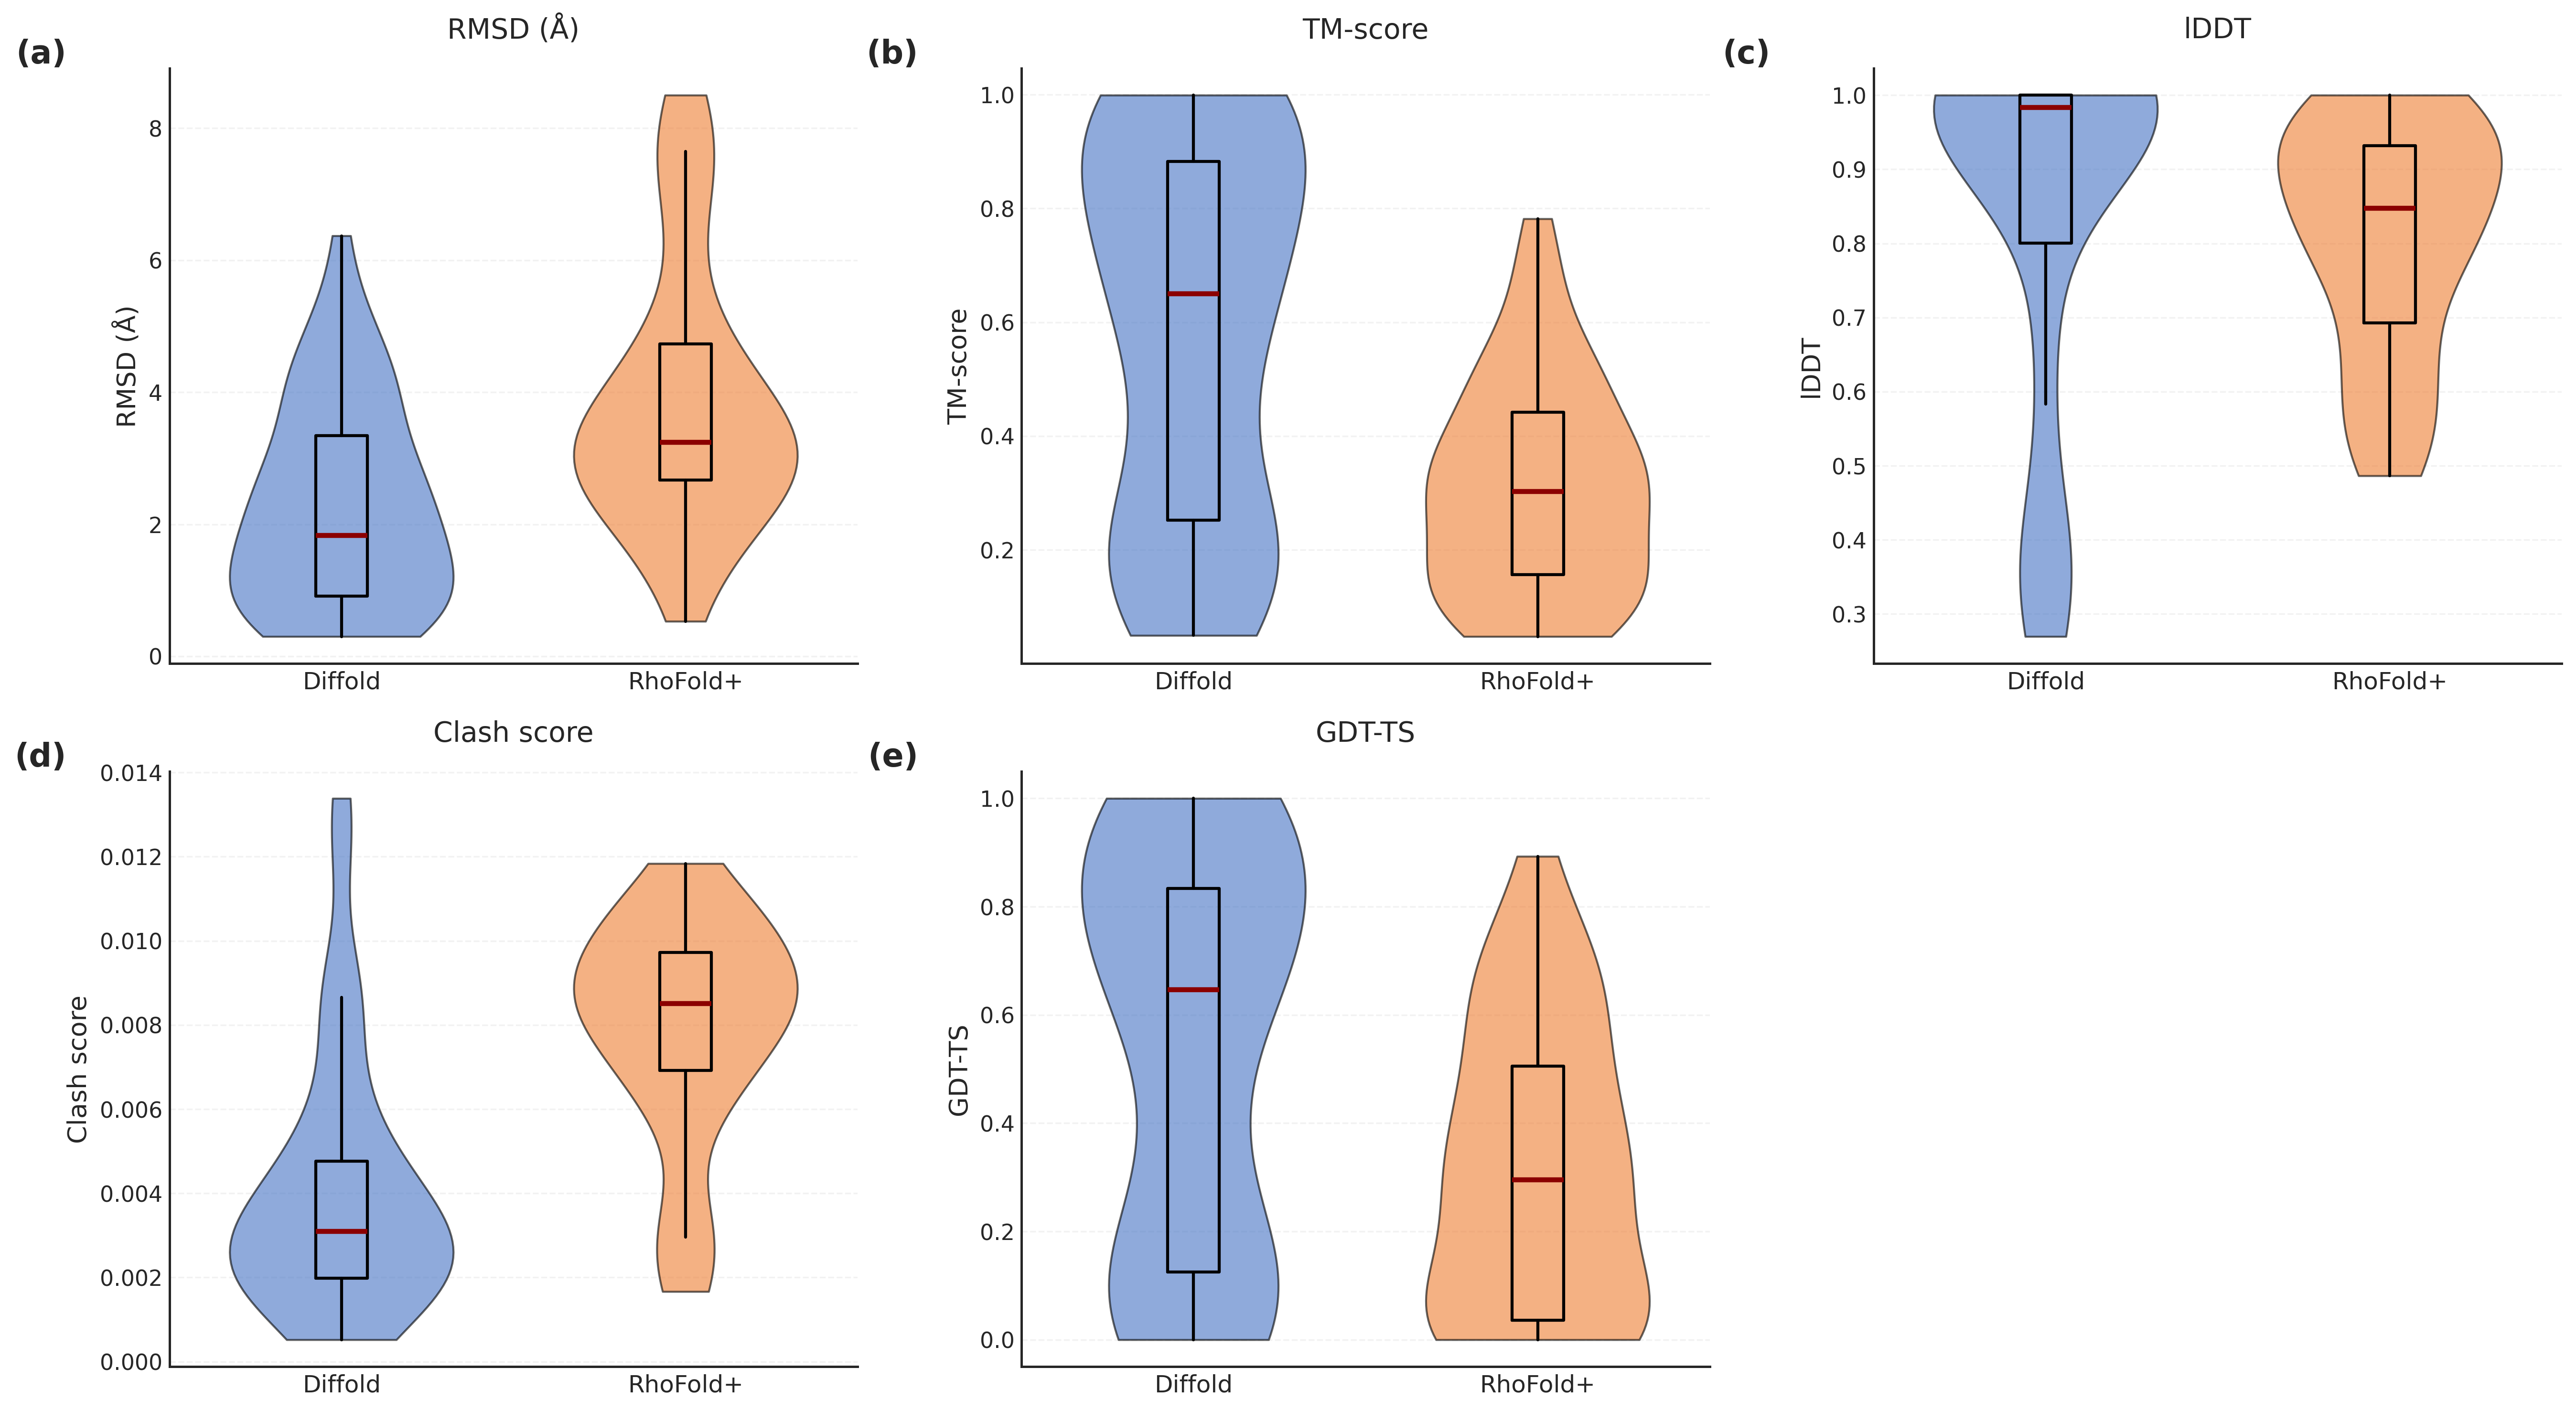
\includegraphics[width=1\linewidth]{img/Performance.png}
    \caption{Overall performance comparison of Diffold and RhoFold+ on the CASP16 and RNA-benchmark test set. Violin plots show metric distributions with boxplots indicating the median and interquartile range: (a) RMSD, (b) TM-score, (c) lDDT, (d) clash score, and (e) GDT-TS}
    \label{fig:performance}
\end{figure}

\begin{figure}
    \centering
    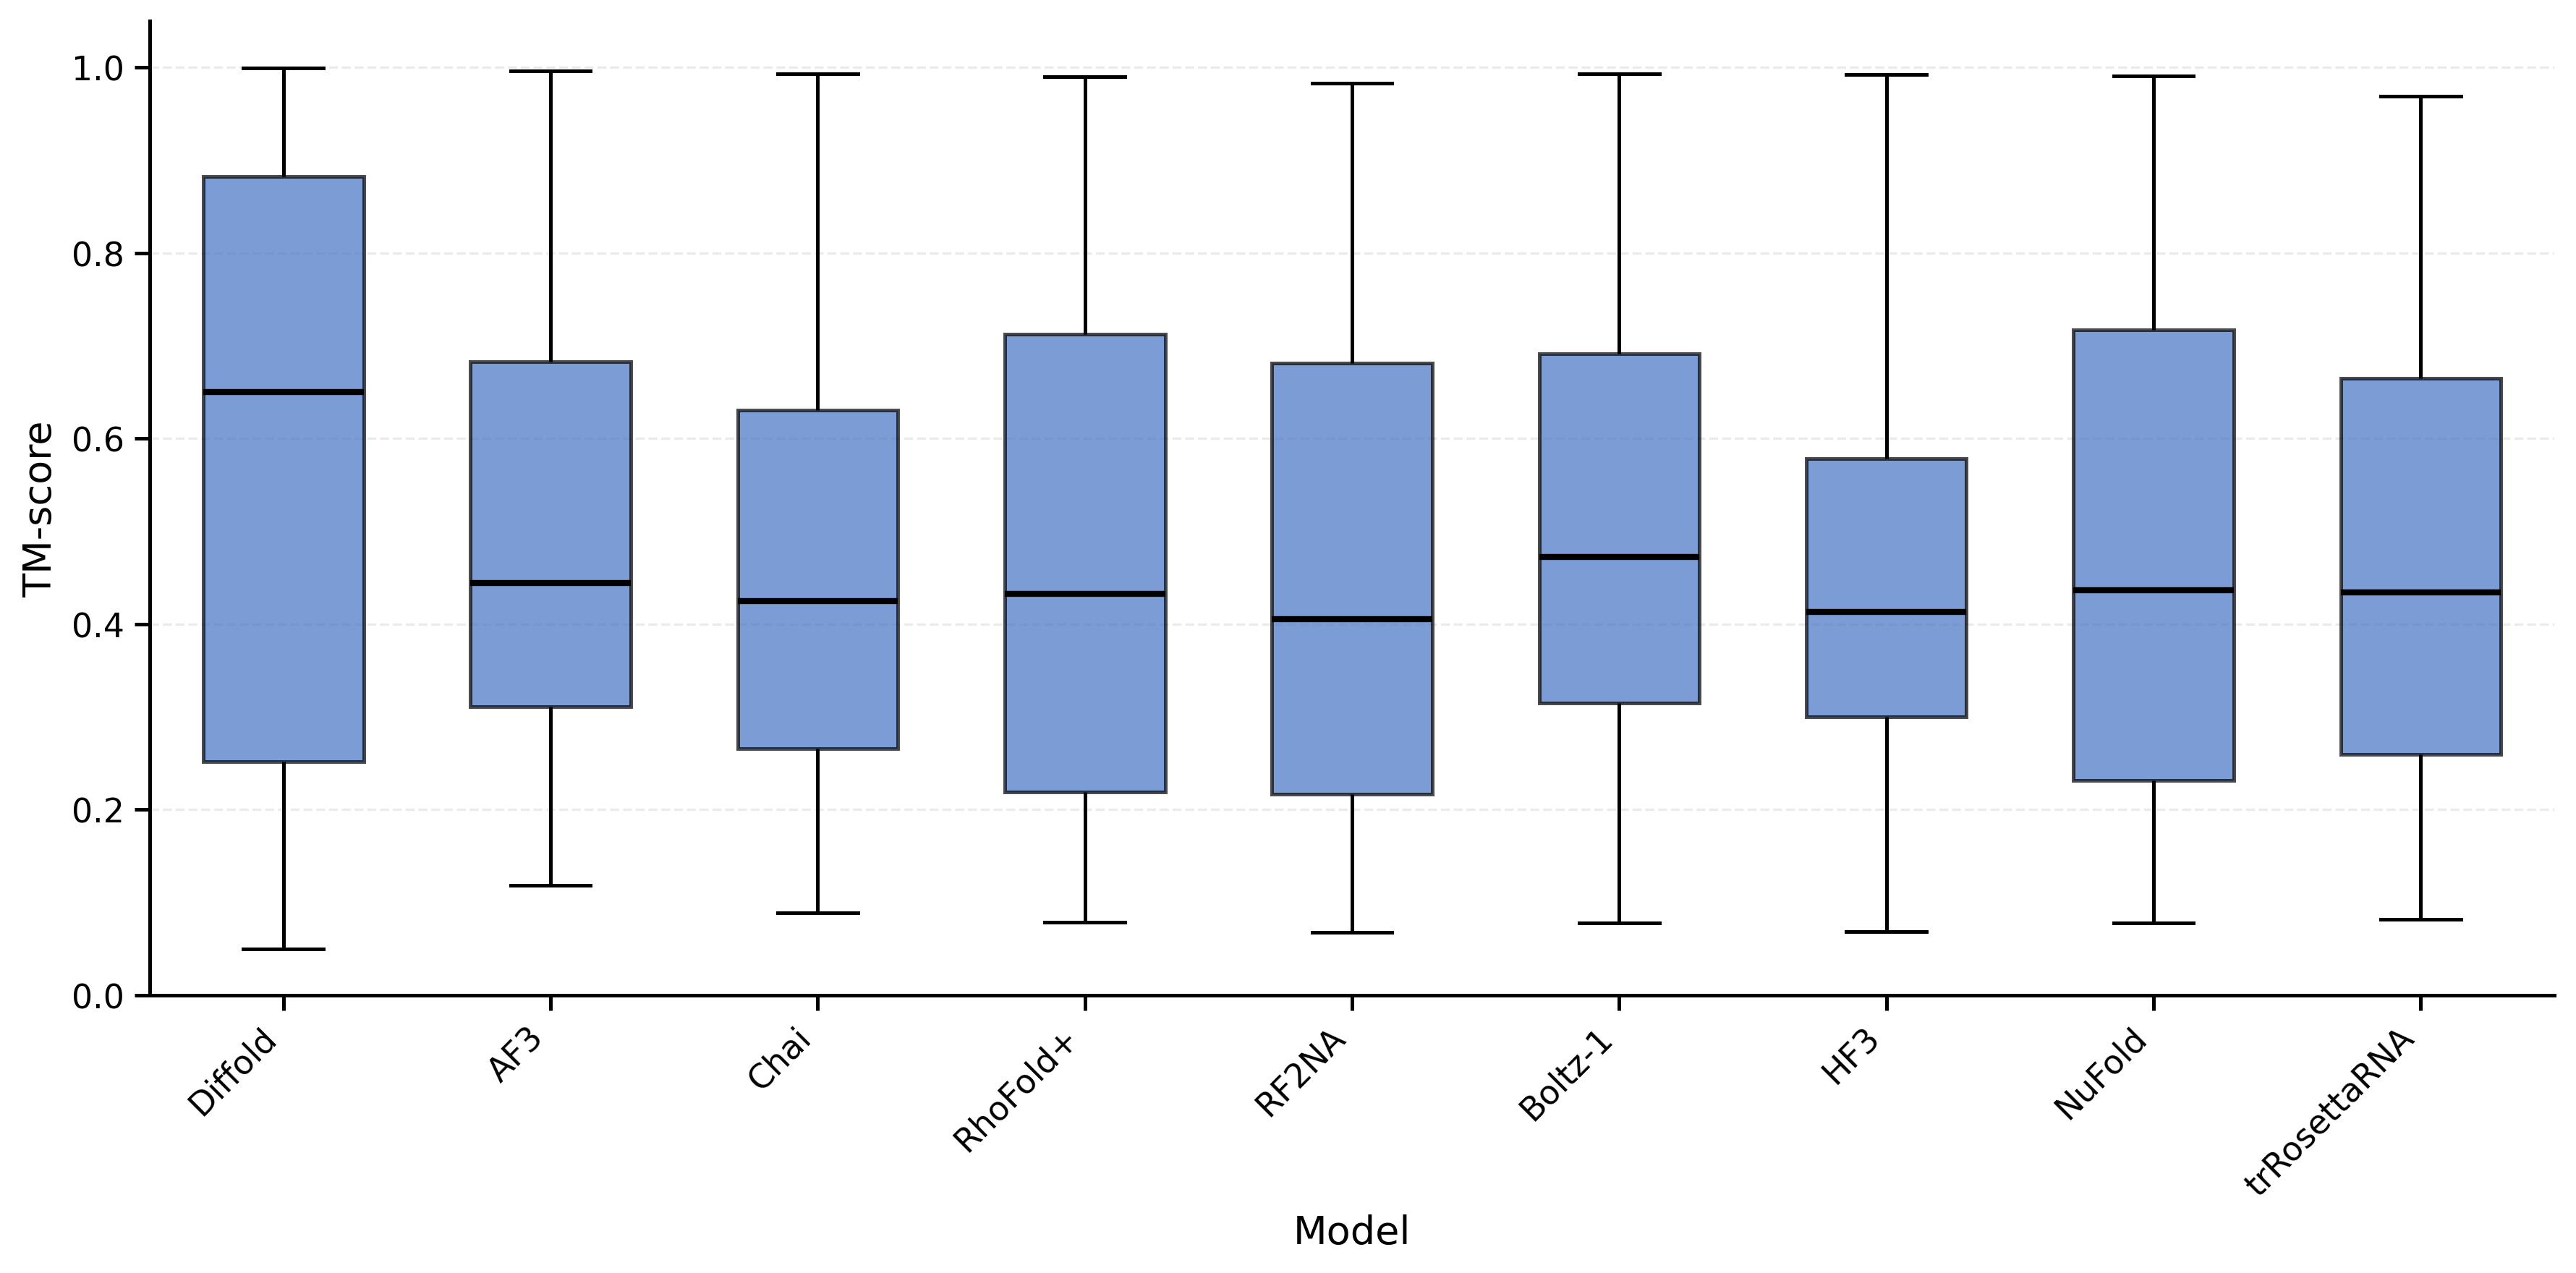
\includegraphics[width=1\linewidth]{img/Models_comparison.png}
    \caption{Cross-model comparison on RNA-Benchmark. TM-score distributions for Diffold and representative baselines}
    \label{fig:tmscore}
\end{figure}

\section{Performance Analysis}

\subsection{Sequence Length Analysis}

Across the combined CASP16 and RNA-benchmark test set, we further examined how prediction quality varies with sequence length (Fig. 4.3). As expected, RhoFold+ shows a clear length-dependent degradation: TM-score decreases with increasing length ($r=-0.440$, $p=7.7\times10^{-4}$), lDDT also decreases ($r=-0.391$, $p=3.1\times10^{-3}$), and GDT-TS exhibits an even stronger negative trend ($r=-0.573$, $p=4.9\times10^{-6}$), while RMSD increases sharply with length ($r=0.928$, $p=2.3\times10^{-24}$). In contrast, Diffold demonstrates markedly weaker length sensitivity for local and distance-based metrics, with near-zero correlations for RMSD ($r=0.011$, $p=0.94$) and lDDT ($r=0.021$, $p=0.88$), and only a mild, non-significant trend for GDT-TS ($r=0.126$, $p=0.35$). Notably, Diffold exhibits a positive correlation between TM-score and sequence length ($r=0.504$, $p=7.5\times10^{-5}$), which is counter to the commonly observed negative relationship in structure prediction. We attribute this phenomenon to a combination of data and model factors: first, Diffold was trained on RNAs with length limited to 16–256 nt, yet maintains stable accuracy on longer targets, suggesting favorable length generalization of the diffusion-based generator beyond the training regime; second, the distribution of test targets is uneven across lengths, and the subset of long RNAs may be enriched for more regular, helix-dominant folds that are comparatively easier to capture at the global topology level, thereby yielding higher TM-scores; third, shorter RNAs can contain highly flexible motifs and sparse evolutionary signal, and TM-score can be more sensitive to small absolute coordinate errors on short chains, which may collectively depress TM-score in the short-length regime. Therefore, while the positive TM-score–length trend should be interpreted with caution given potential composition bias in the test set, the overall pattern supports the conclusion that Diffold is substantially less affected by increasing sequence length than RhoFold+ and generalizes well to longer RNAs despite the absence of above 256 nt examples during training.

\begin{figure}
    \centering
    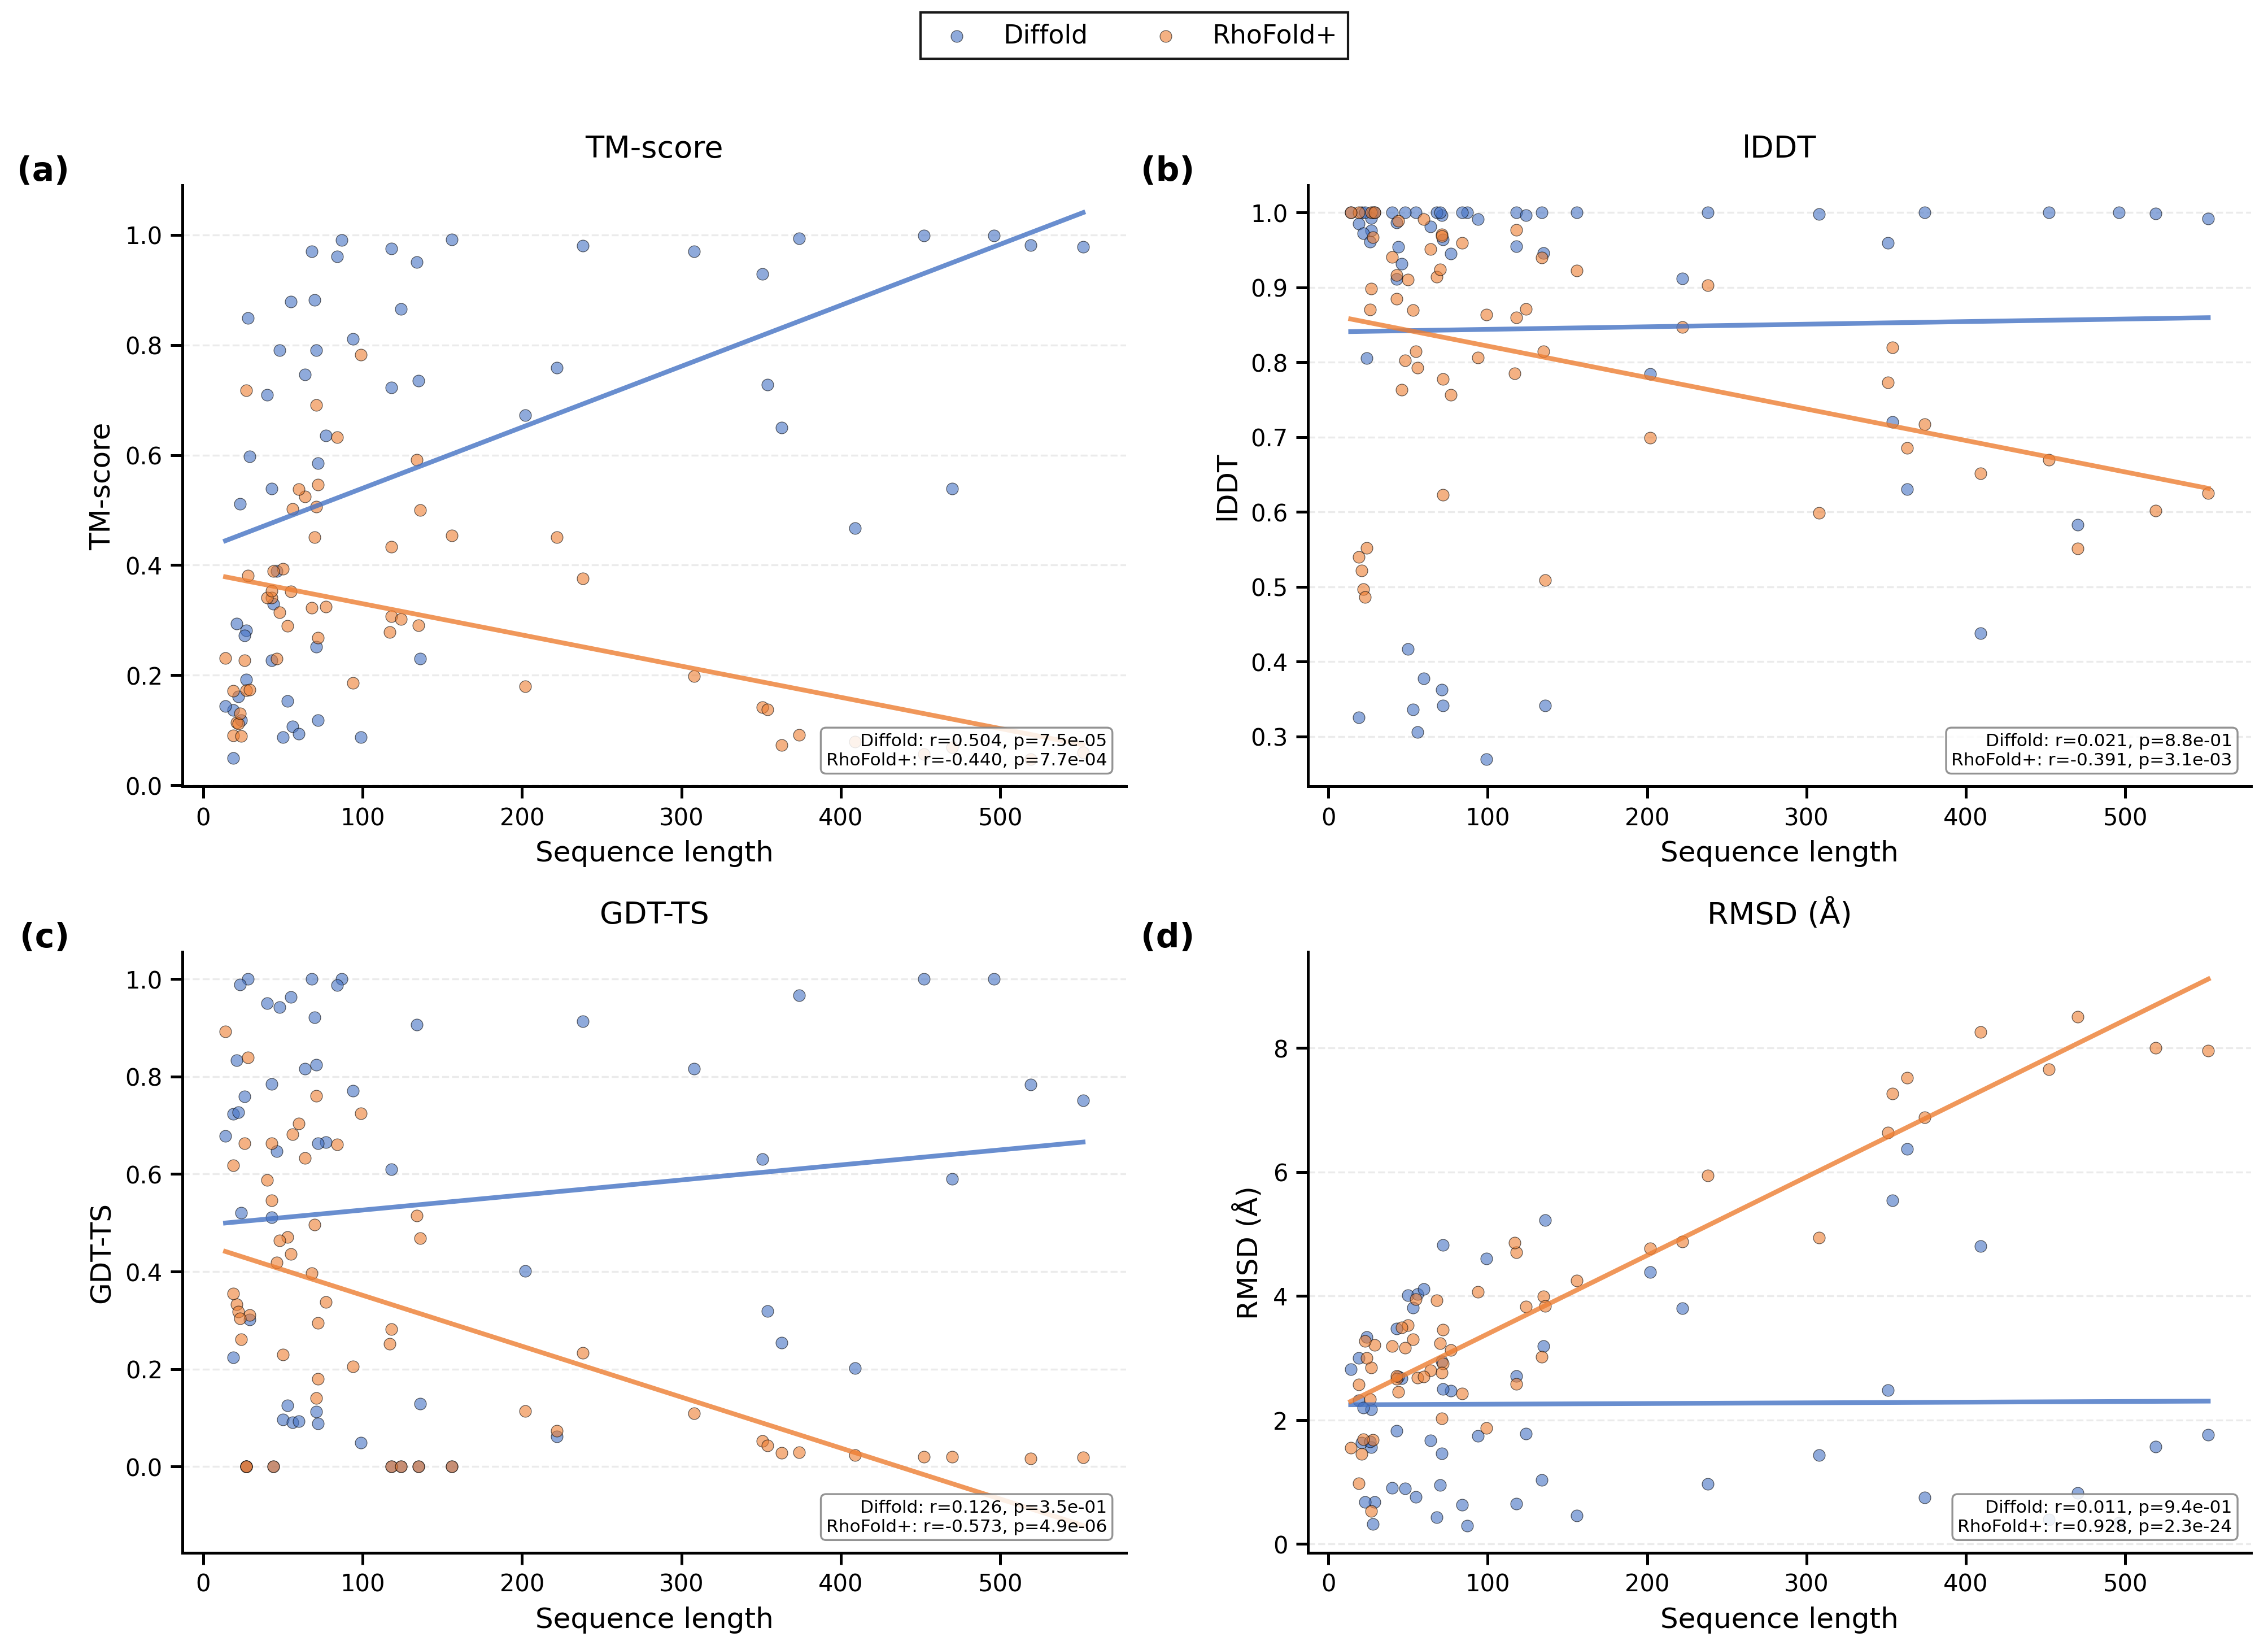
\includegraphics[width=1\linewidth]{img/Length_analysis.png}
    \caption{Relationship between sequence length and prediction metrics. Scatter plots report TM-score, lDDT, GDT-TS, and RMSD versus sequence length for Diffold and RhoFold+, with linear regression trends and correlation statistics.}
    \label{fig:length vs performance}
\end{figure}

\subsection{Dataset Dependence Analysis}

\begin{figure}
    \centering
    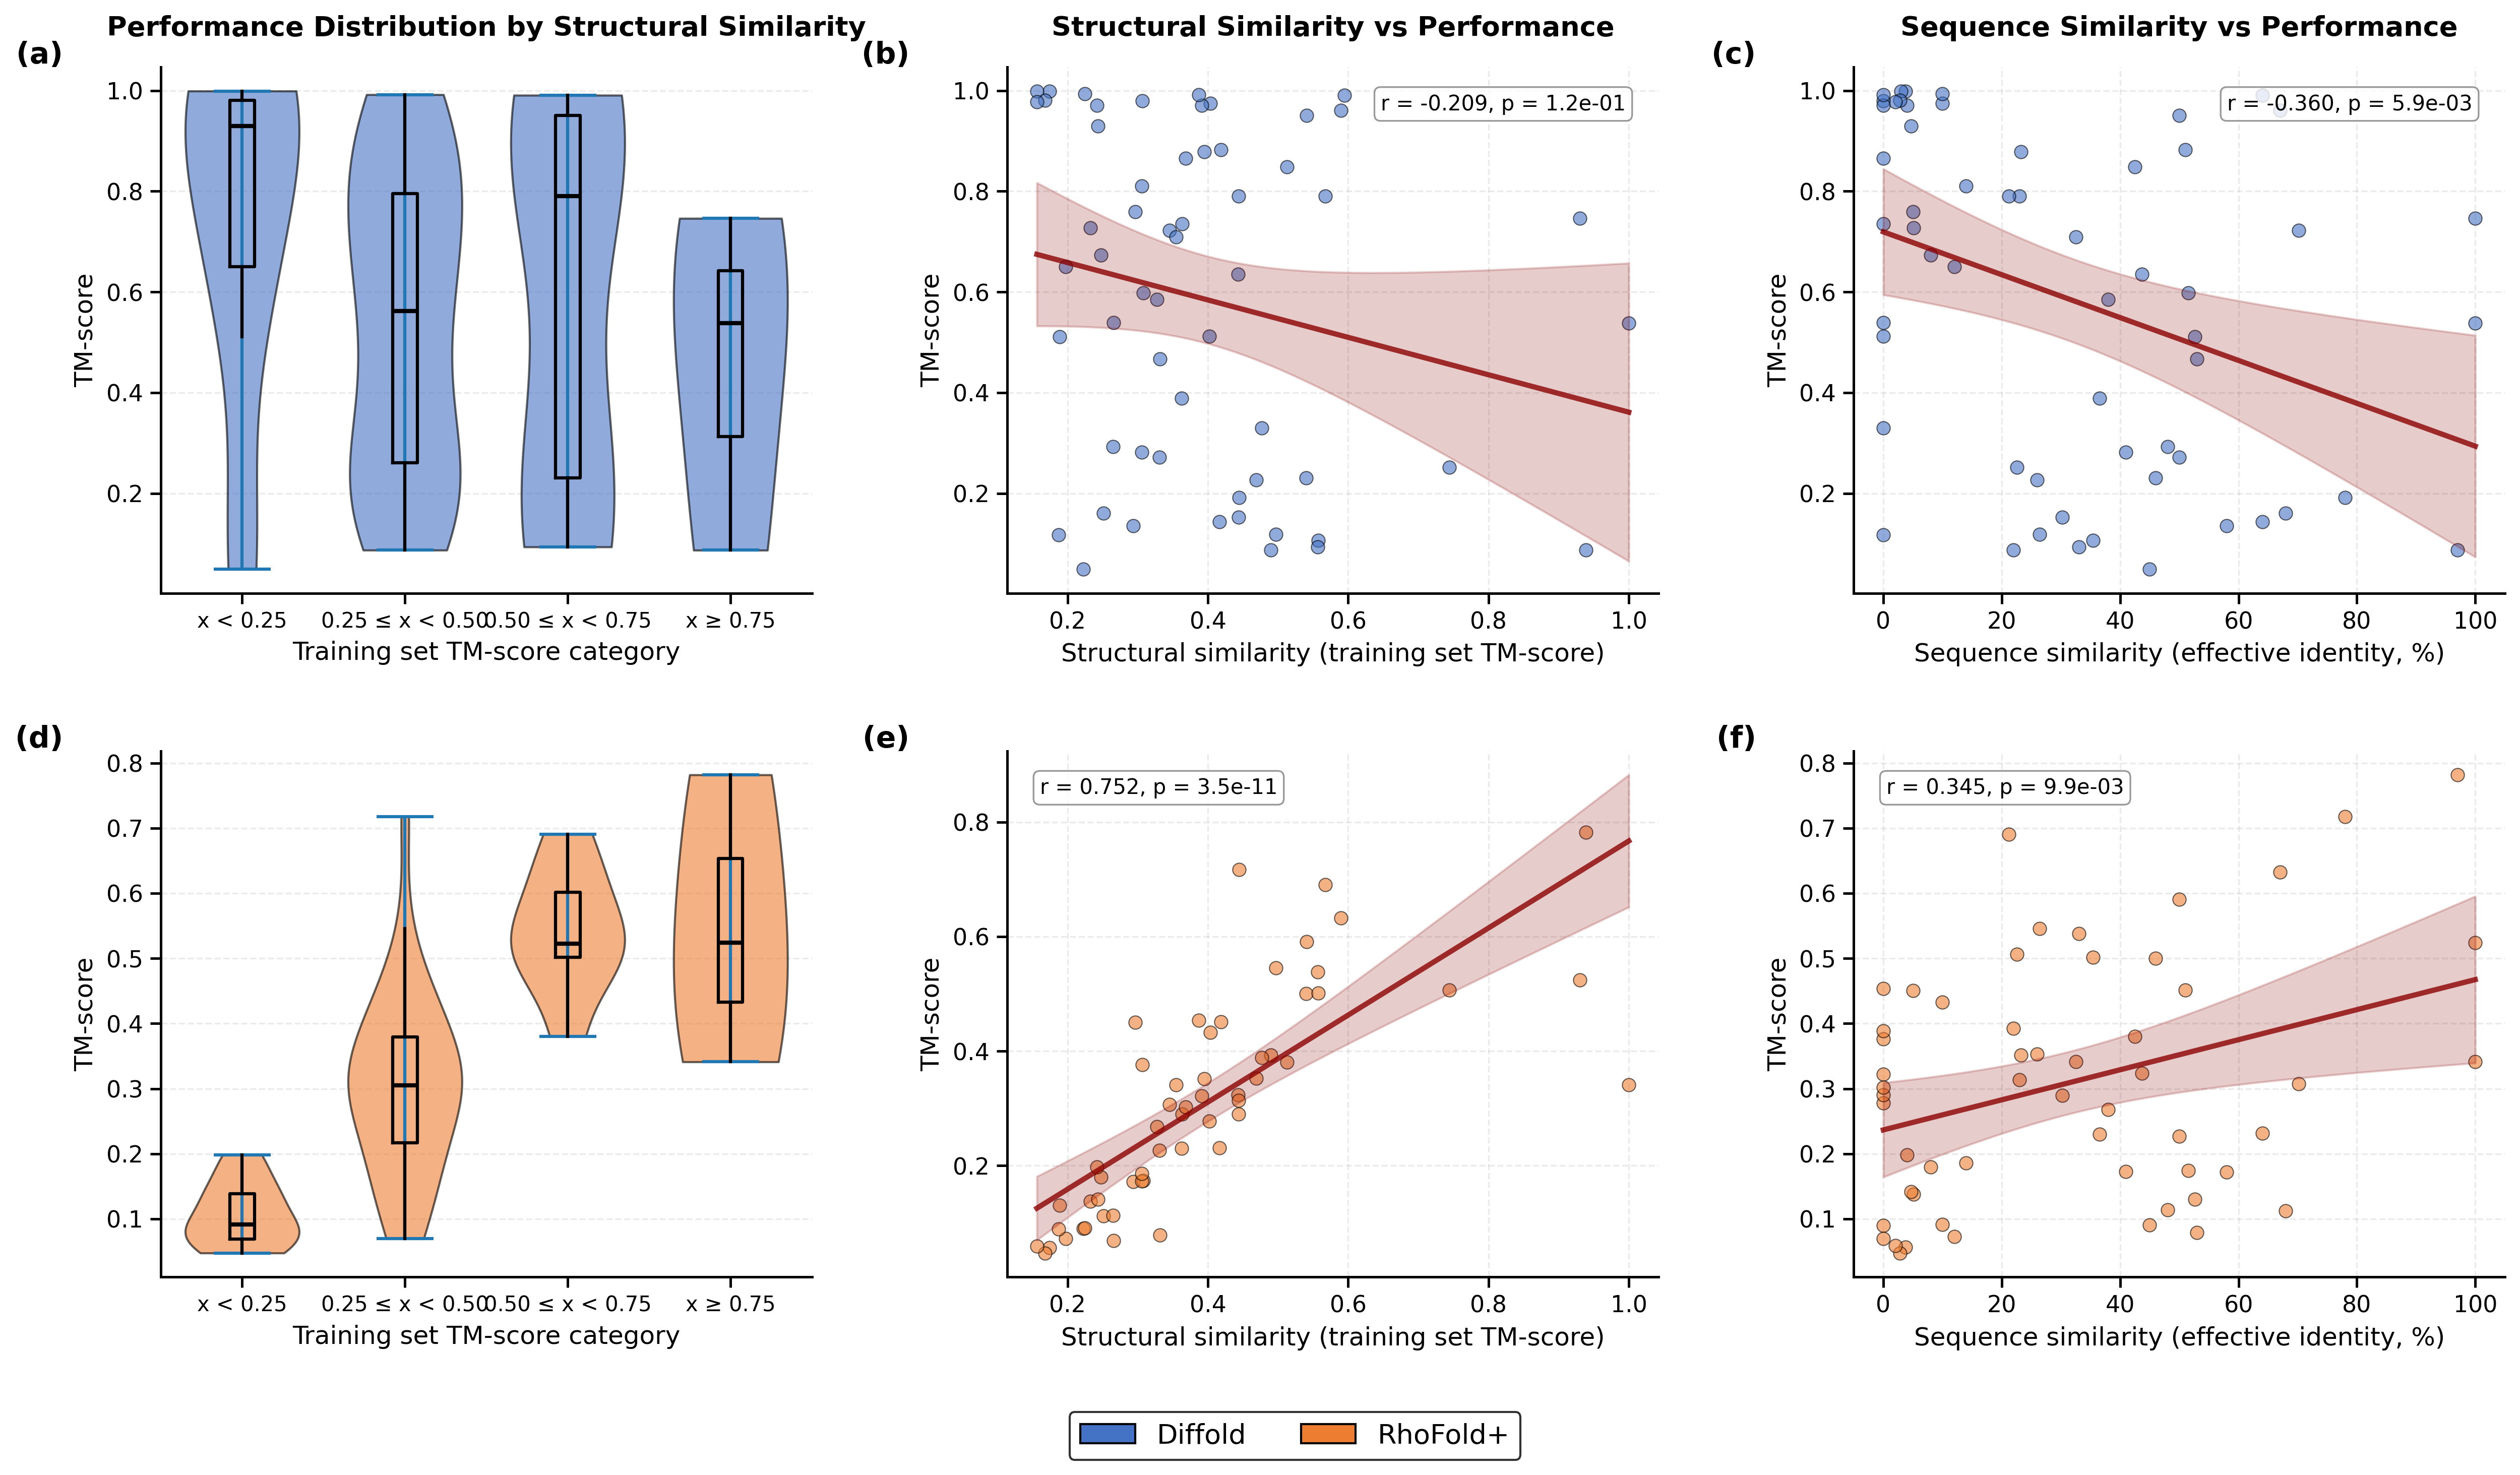
\includegraphics[width=1\linewidth]{img/new_dependence_analysis.png}
    \caption{Performance versus train–test similarity. (a–c) Diffold and (d–f) RhoFold+ on the test set. Train–test structural similarity is defined as the maximum TM-score of each test target to any training structure, and sequence similarity as the maximum BLAST effective identity to any training sequence. Violin plots show performance stratified by bins; scatter plots show per-target performance versus similarity (Pearson $r$, $p$ shown).}
    \label{fig:dependence}
\end{figure}

To assess data independence and potential memorization effects, we analyzed train--test similarity at both the structural and sequence levels (Fig.~4.4). For each test target $T$, we quantified its nearest-neighbor structural proximity to the training set as $\mathrm{Indep}_{\mathrm{struct}}(T)$, defined by the maximum TM-score between the native structure of $T$ and any native training structure, and examined how prediction accuracy varies with this similarity. Diffold shows no significant dependence on training-set structural proximity, with a weak and non-significant correlation ($r=-0.209$, $p=1.2\times10^{-1}$; Fig.~4.4b) and broadly comparable TM-score distributions across structural similarity bins (Fig.~4.4a). In contrast, RhoFold+ exhibits a strong positive association between performance and training-set structural similarity ($r=0.752$, $p=3.5\times10^{-11}$; Fig.~4.4e), and its TM-score increases substantially as the closest training neighbor becomes more similar. This pattern suggests that RhoFold+ benefits more from the presence of structurally similar examples in the training set, whereas Diffold is less tied to nearby structural neighbors.

We further repeated the analysis using the nearest-neighbor sequence proximity $\mathrm{Indep}_{\mathrm{seq}}(T)$, computed as the maximum BLAST effective identity between each test sequence and any training sequence. Notably, Diffold exhibits a negative association between performance and sequence similarity ($r=-0.360$, $p=5.9\times10^{-3}$; Fig.~4.4c), while RhoFold+ shows a modest but significant positive association ($r=0.345$, $p=9.9\times10^{-3}$; Fig.~4.4f). A likely explanation for this apparent anomaly is that, for RNA, sequence proximity is an imperfect surrogate for structural proximity: homologous RNAs may share conserved motifs yet differ in global fold, domain organization, or long-range/pseudoknotted interactions, so targets with high $\mathrm{Indep}_{\mathrm{seq}}$ can remain structurally novel and difficult. Moreover, BLAST is local-alignment based; high effective identity can still be driven by a conserved segment within a longer or multi-domain construct, inflating $\mathrm{Indep}_{\mathrm{seq}}$ without implying an easier whole-structure prediction problem. A third possibility is conflicting supervision among near-homologs in the training set (e.g. different constructs, bound states, or alternative conformations), which yields a multi-modal conditional distribution; a diffusion generator that models a broader ensemble may distribute probability mass across modes, reducing the likelihood of matching the single reference structure used for evaluation. Finally, $\mathrm{Indep}_{\mathrm{seq}}$ may correlate with confounders such as sequence length or structural complexity; if high-$\mathrm{Indep}_{\mathrm{seq}}$ targets are systematically harder, a negative correlation can emerge even in the absence of memorization. Taken together, the structural and sequence diagnostics consistently indicate that RhoFold+ benefits more from train-test proximity, whereas Diffold maintains competitive accuracy even when structurally distant from the training set, supporting stronger generalization and improved data independence under this evaluation protocol.


\section{Case Study}

\subsubsection{Case1: 8UYG}

For 8UYG, a 135-nt RNA target, we observed that directly generated all-atom coordinates occasionally violate covalent geometry along the RNA backbone, most notably the $\text{O3}'–\text{P}$ phosphodiester bonds, resulting in apparent chain breaks. Quantitatively, before relaxation, 75 $\text{O3}'–\text{P}$ bonds exceeded 2.0 $\text{\AA}$ in length, whereas after AMBER-based relaxation this number decreased to 1, indicating that force-field energy minimization effectively repairs local bond-length pathologies while preserving the overall fold. This case supports the use of AMBER relax as a practical post-processing step to improve the chemical completeness and physical plausibility of diffusion-generated RNA structures, especially when bond-length constraints are not explicitly enforced during generation.


\begin{figure}[H]
    \centering
    % ----- image 1 -----
    \begin{minipage}{0.48\linewidth}
        \centering
        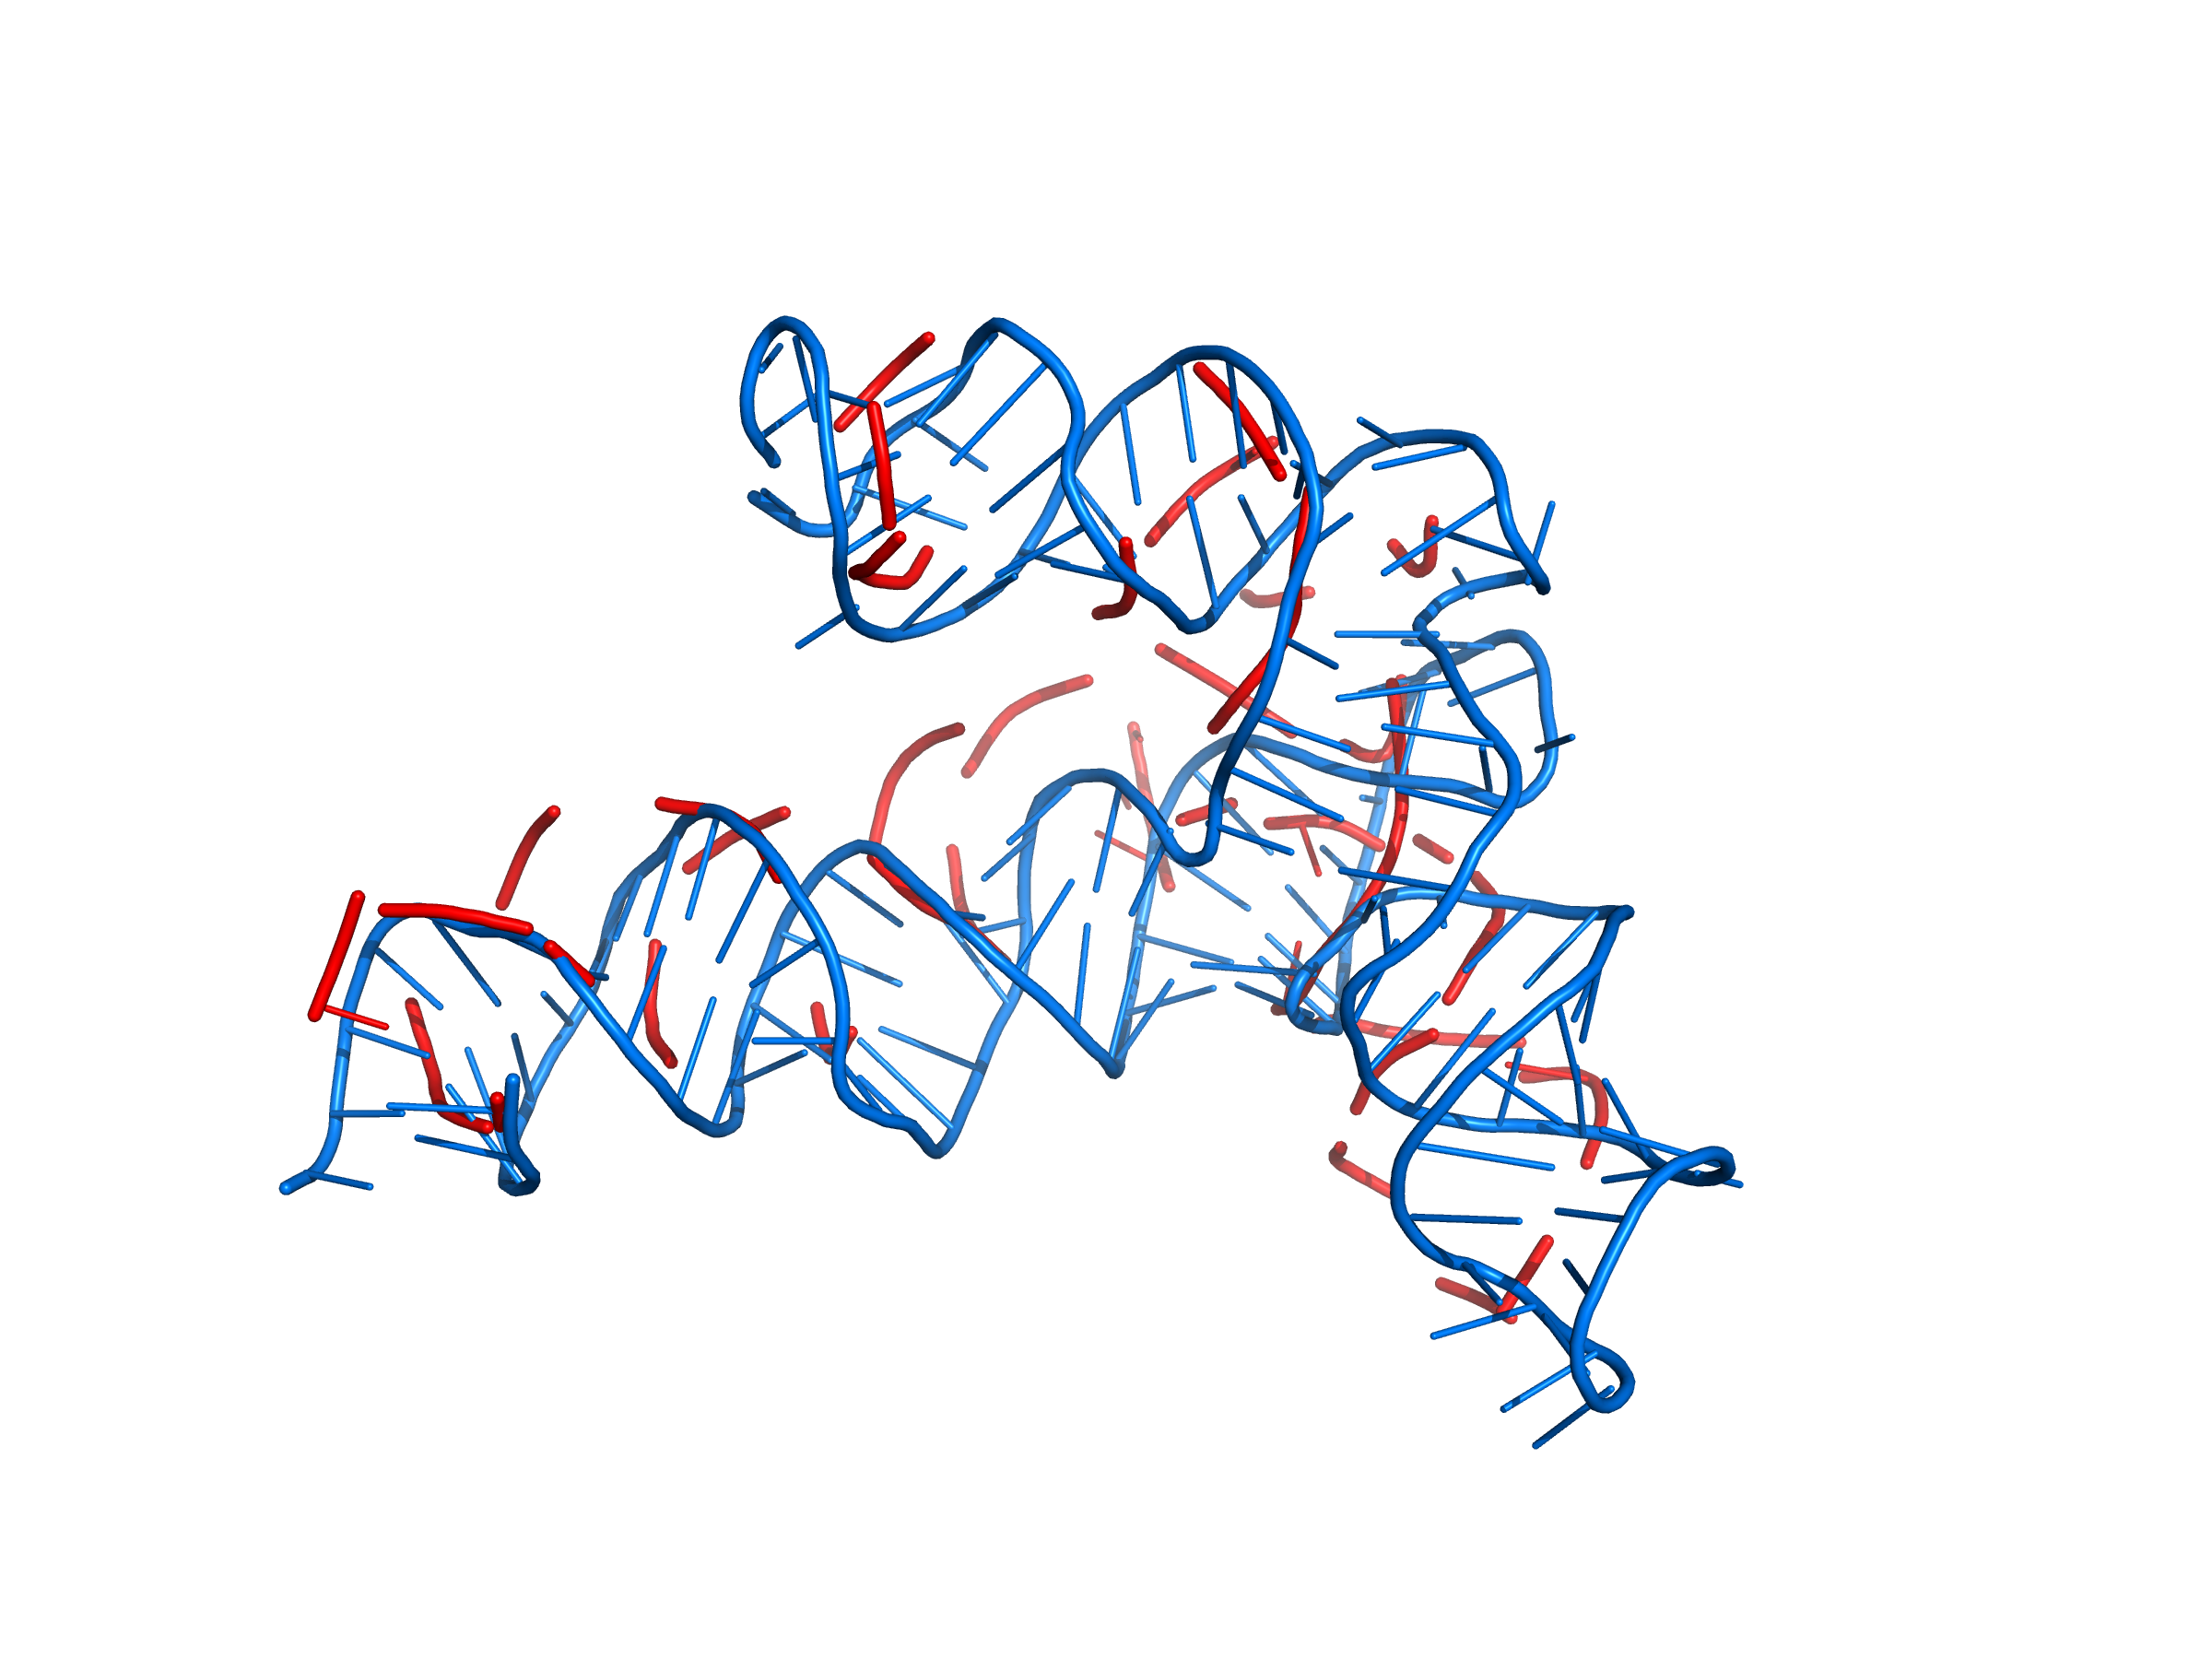
\includegraphics[width=\linewidth]{img/8uyg_pred_relaxed.png}
        \par (a)
    \end{minipage}
    \hfill
    % ----- image 2 -----
    \begin{minipage}{0.48\linewidth}
        \centering
        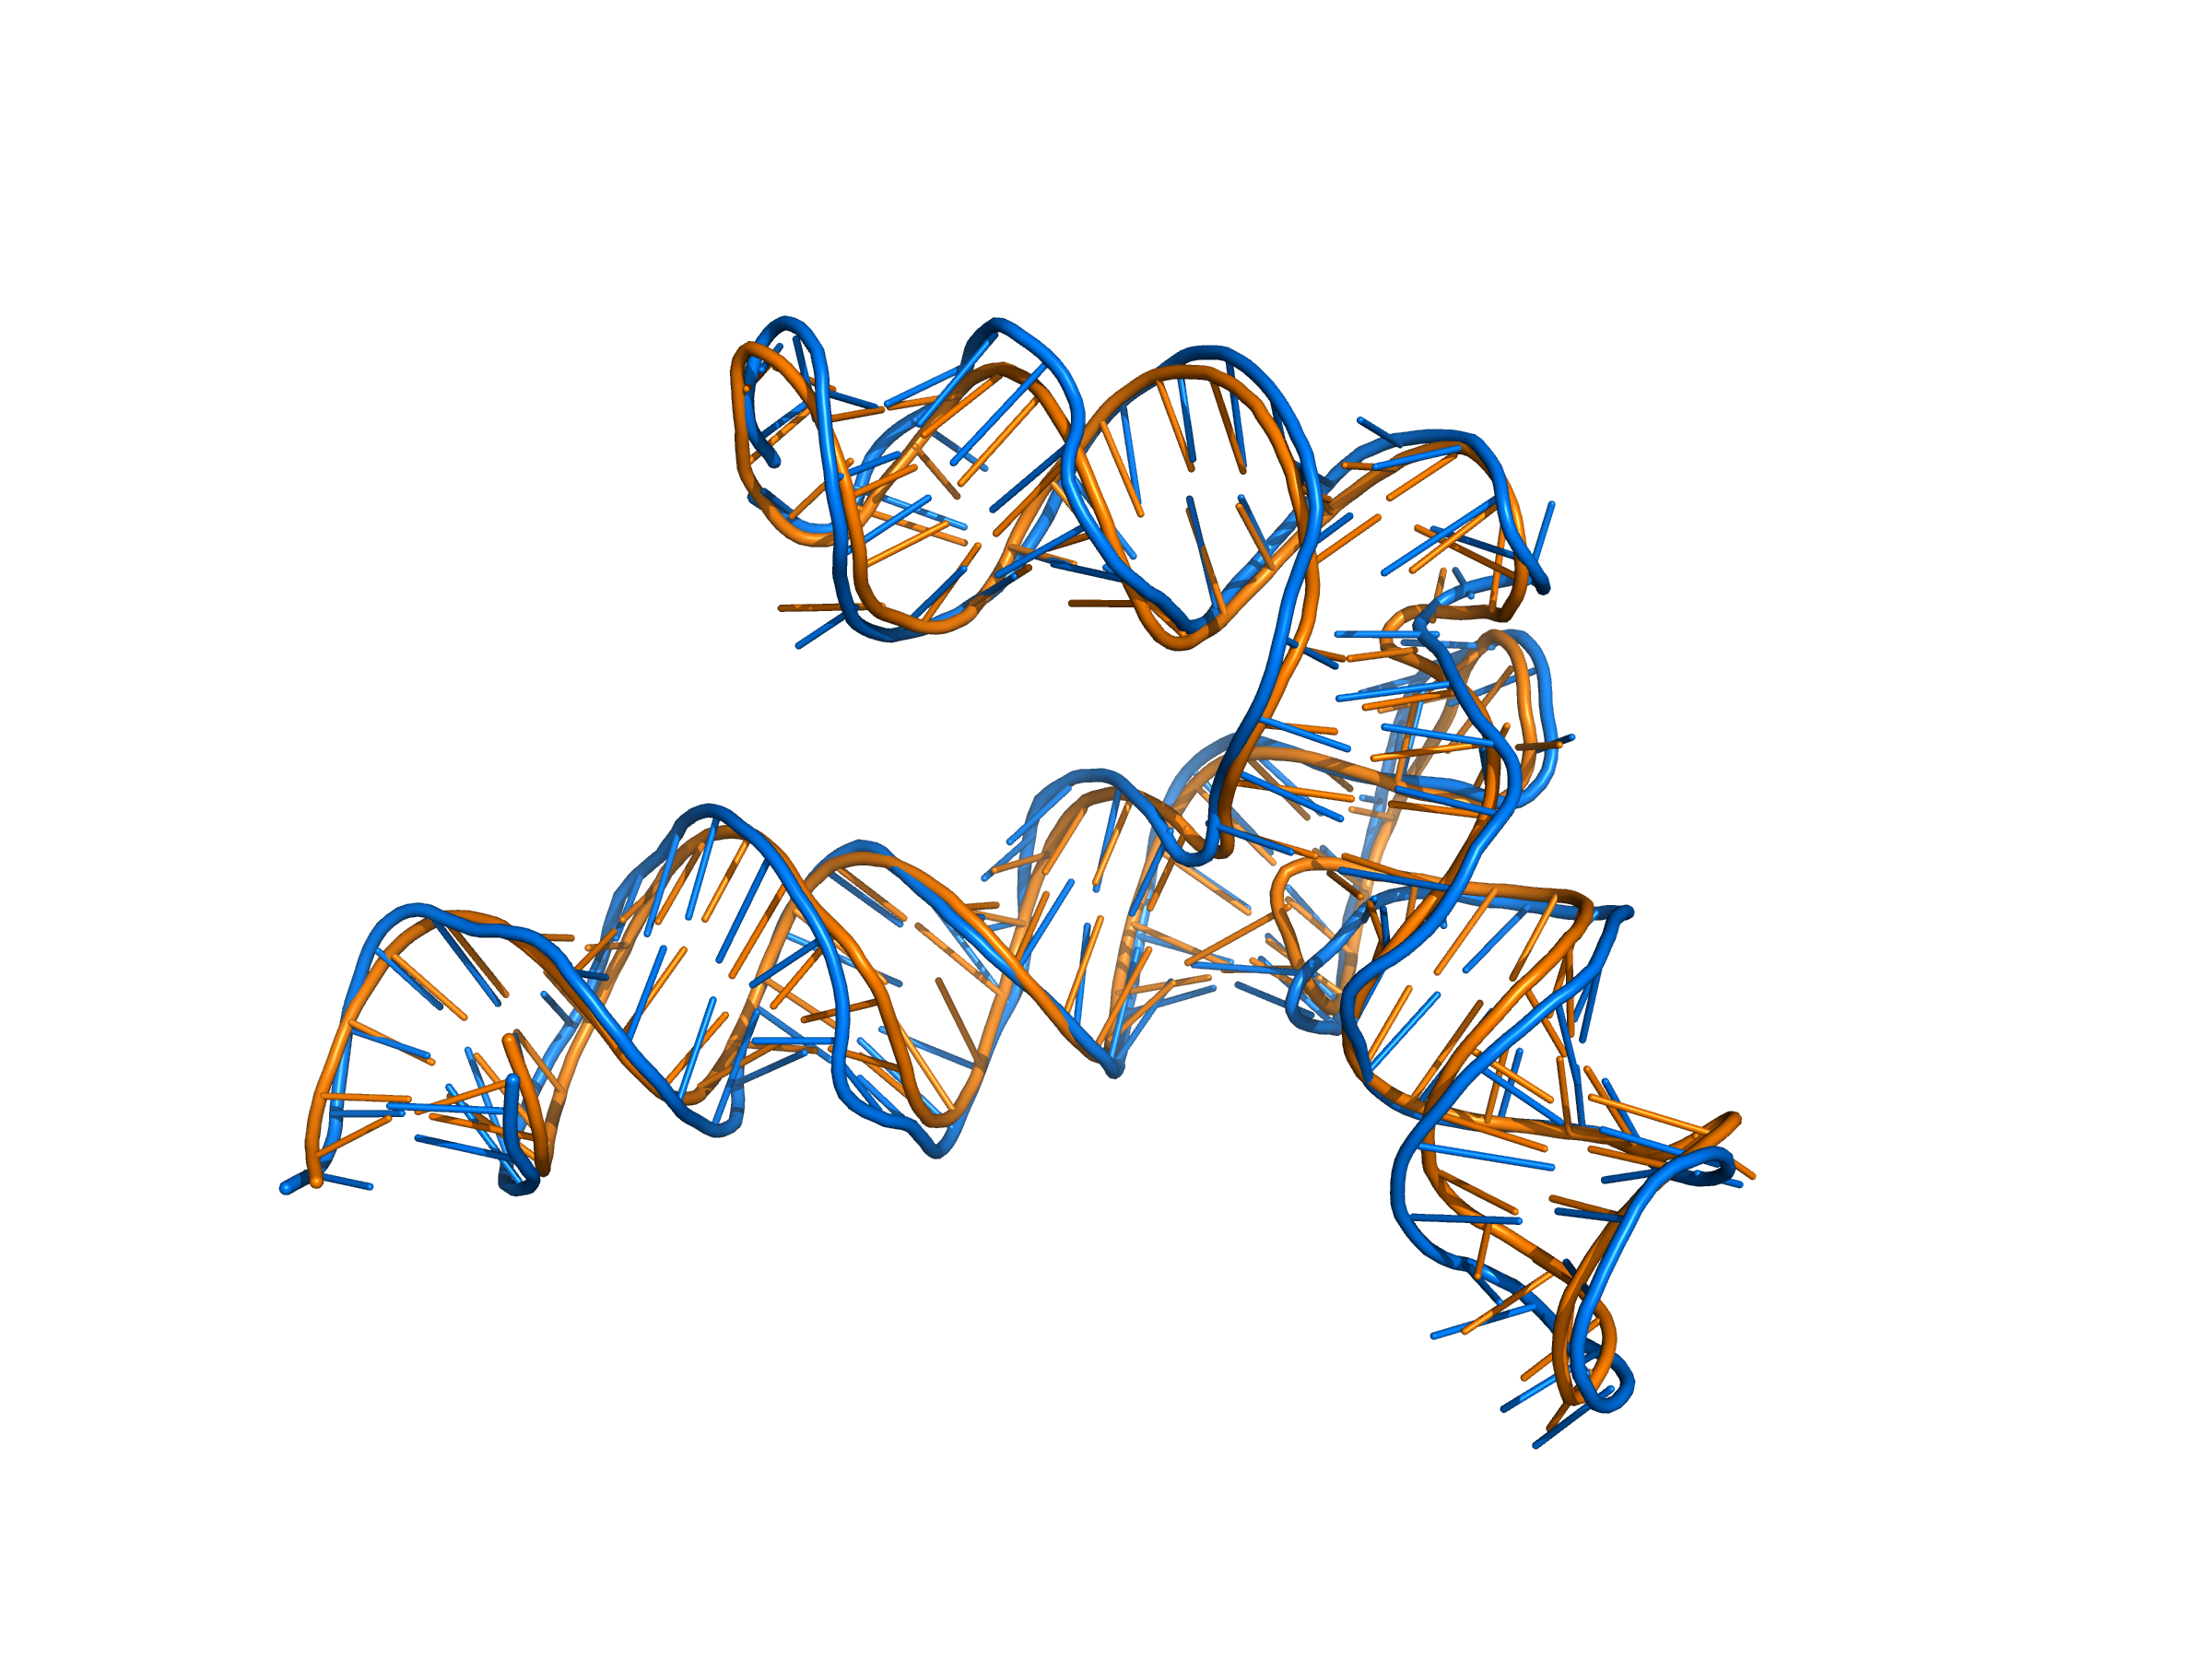
\includegraphics[width=\linewidth]{img/8uyg_pred_native.png}
        \par (b)
    \end{minipage}
    \caption{Structural alignment for PDB 8UYG before and after relaxation.
(a) Overlay of the unrelaxed prediction (red) with the native structure (blue).
(b) Overlay of the relaxed prediction (orange) with the native structure (blue).}
    \label{fig:8uyg}
\end{figure}

\begin{figure}[!htbp]
    \centering
    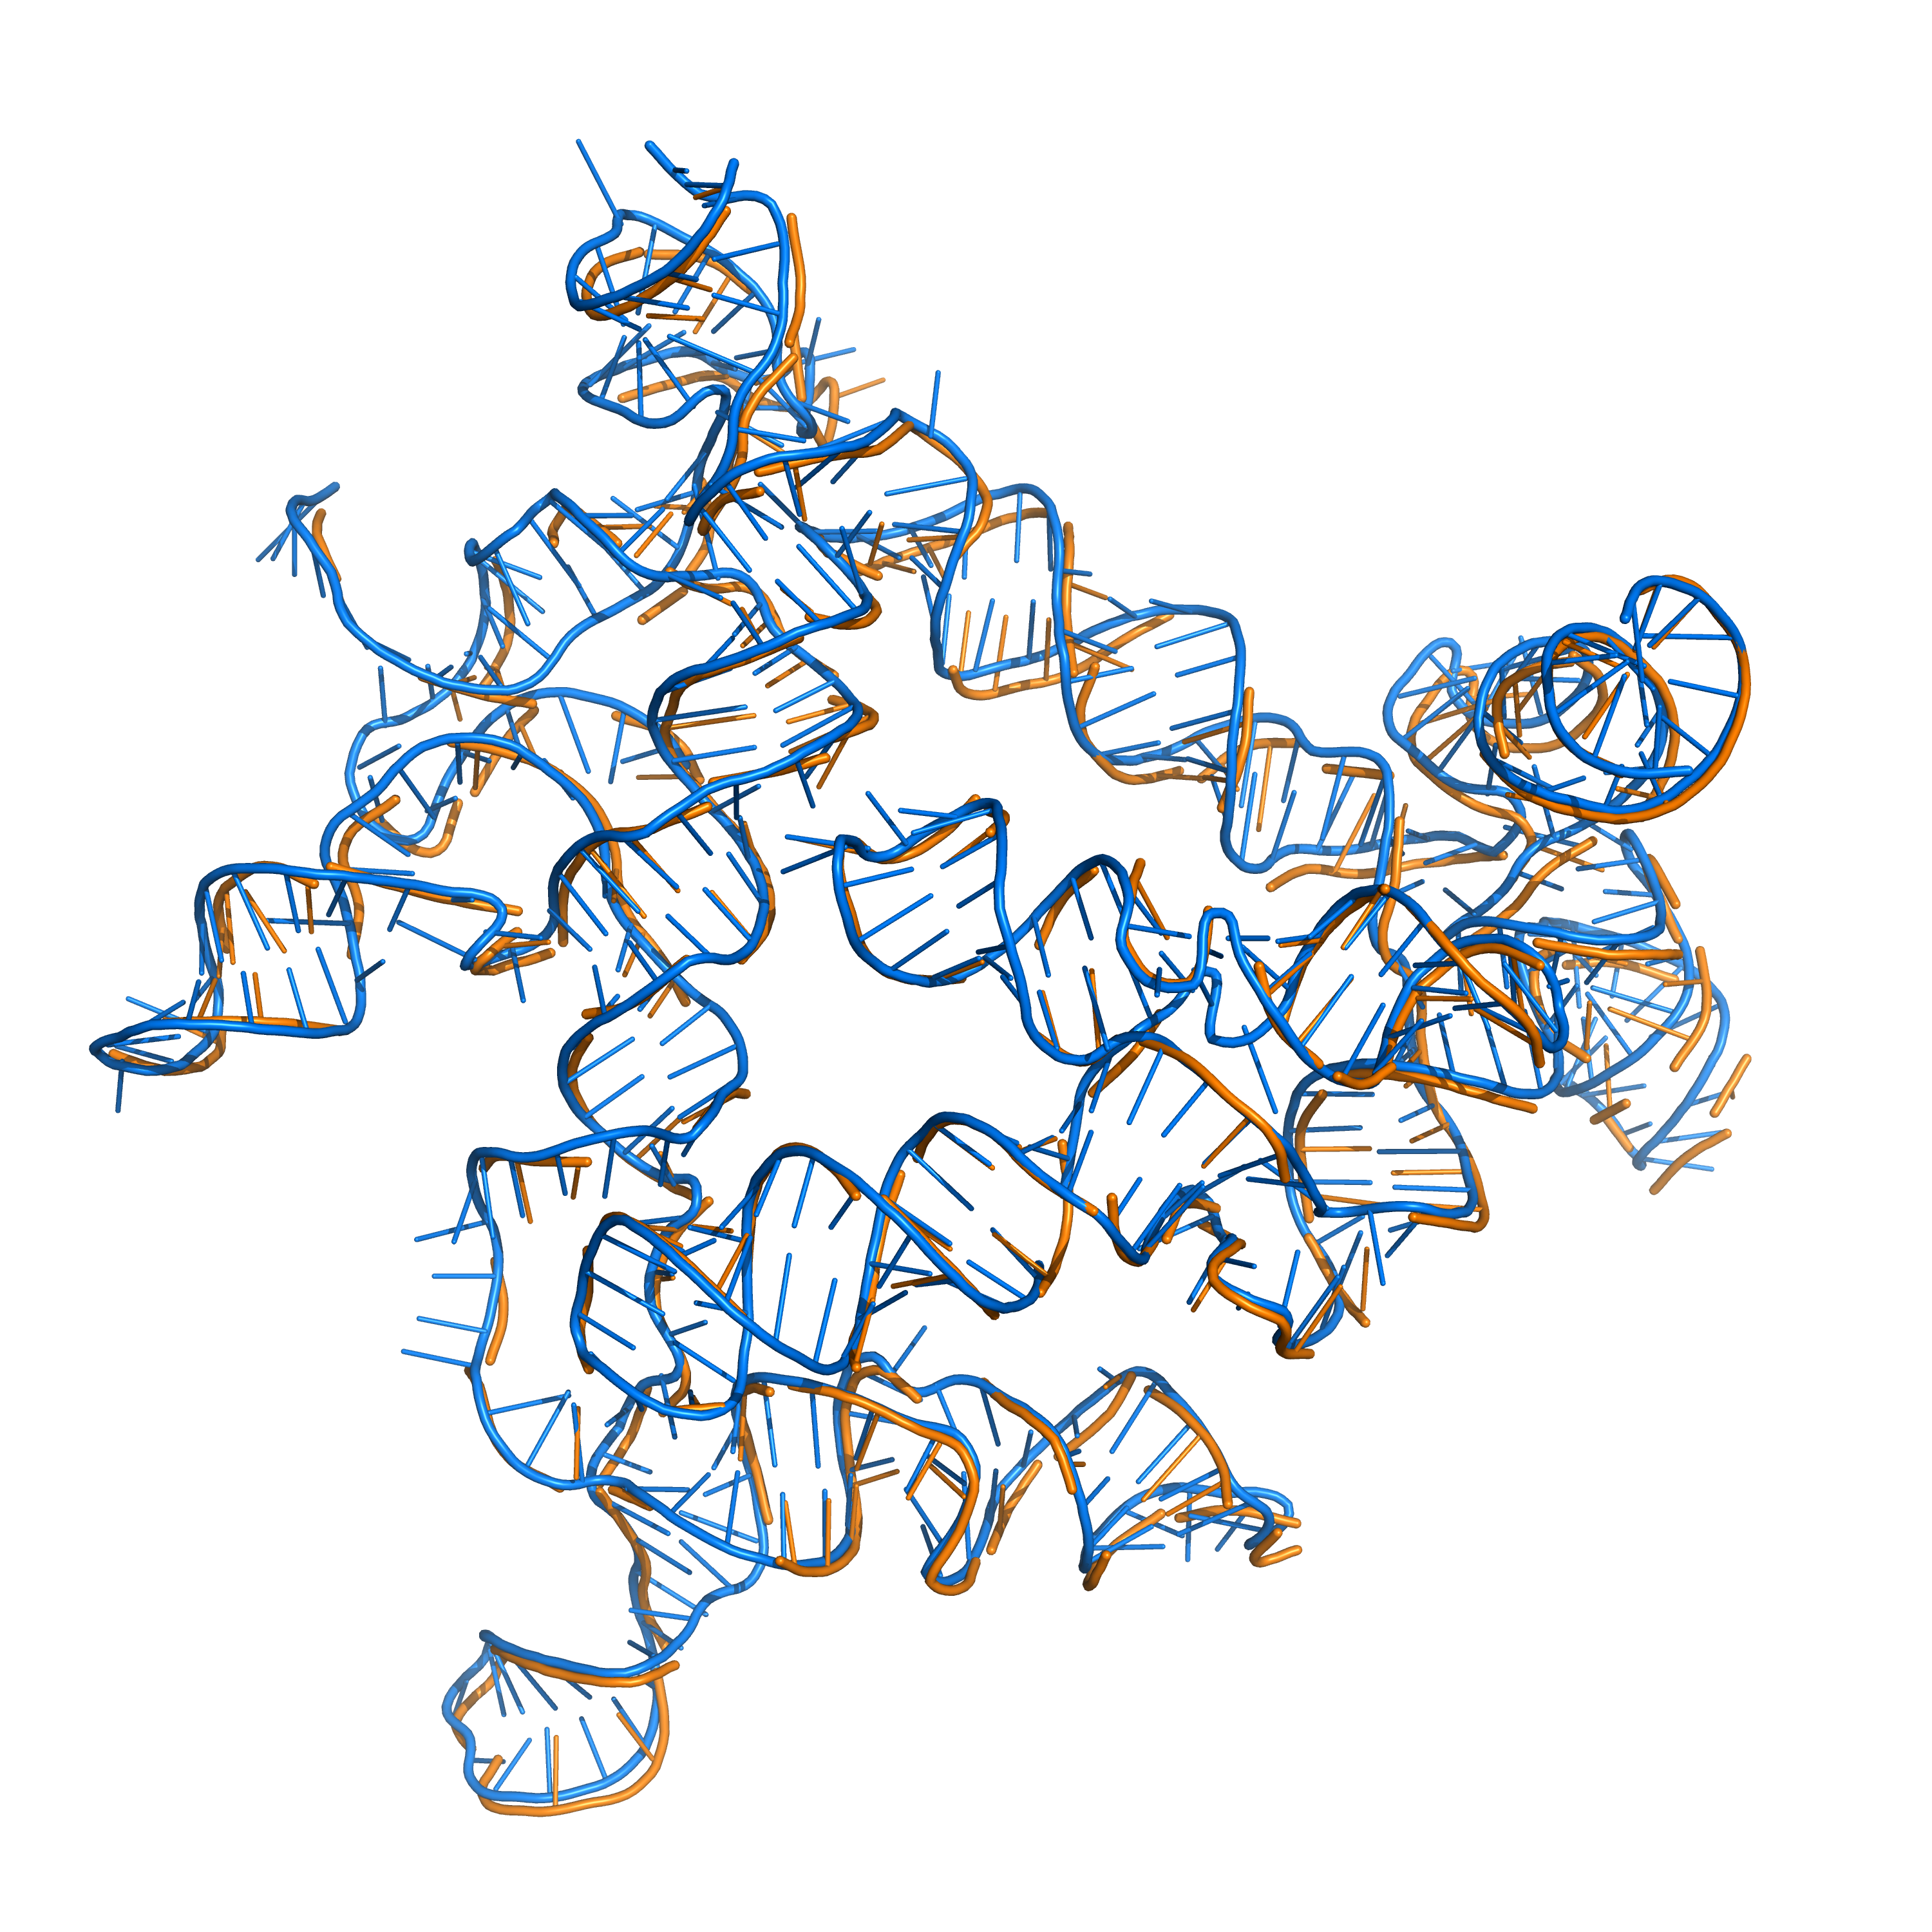
\includegraphics[width=0.5\linewidth]{img/R1283v2_pred_native.png}
    \caption{Structural alignment for R1283v2 (PDB 9J3R).
Overlay of the predicted structure (orange) with the native structure (blue).}
    \label{fig:placeholder}
\end{figure}

\subsubsection{Case2: 9J3R(R1283v2)}

The target R1283v2 corresponds to a long RNA (452 nt) represented by PDB 9J3R. On this target, RhoFold+ fails to recover the native topology, yielding a near-random alignment with TM-score 0.034, while Diffold achieves an almost native-quality reconstruction with TM-score 0.994. This striking gap is notable because the training regime constrains the RNA length to at most 256 nt, implying that Diffold can extrapolate beyond the training length regime and maintain long-range structural coherence at a scale of several hundred nucleotides.

At the same time, this case exposes a systematic geometry issue of Diffold: it tends to predict slightly elongated covalent distances along the backbone, most prominently the O3$'$\!--P linkage. For short RNAs, the subsequent relaxation step is highly effective at correcting these local bond-geometry deviations, restoring chain continuity without materially affecting the global fold. In contrast, for long targets such as R1283v2, the same bias accumulates over hundreds of nucleotides and manifests as widespread backbone discontinuities. Once many O3$'$\!--P distances exceed the bonding threshold, standard relax procedures provide only limited benefit: they can smooth local sterics and adjust nearby torsions, but they typically cannot globally re-establish covalent connectivity across numerous breaks without explicit bond-length restraints or dedicated connectivity-repair operations. Consequently, relaxation remains effective for short molecules but becomes nearly ineffective for long RNAs, even when the overall topology is largely correct.

Overall, R1283v2 highlights a separation between Diffold's strong global generalization and a length-amplified local backbone-geometry bias, suggesting that improving covalent-geometry constraints during generation or adding constraint-aware refinement will be important for robust long-RNA modeling.



\subsubsection{Case3: 7WIA}

In contrast, 7W1A represents a challenging failure case: although its nearest training-set structural neighbor reaches a maximum TM-score of 0.81, Diffold attains only TM-score 0.162, whereas RhoFold+ achieves 0.661 on the same target. This discrepancy indicates that training-set proximity alone is insufficient to guarantee successful generation, especially for compact, topology-sensitive RNAs.

A key observation is that Diffold's prediction for 7W1A exhibits severe backbone fragmentation (widespread chain discontinuities), such that the model produces locally plausible fragments but fails to assemble a single continuous fold. In this regime, standard relaxation offers limited benefit because it can smooth local sterics and adjust torsions, yet it cannot reliably re-establish covalent connectivity across many breaks without explicit bond-length restraints or dedicated connectivity-repair steps. Consequently, the evaluation against a single native reference yields a very low TM-score even if some local motifs are partially correct.

From a biological and biophysical perspective, 7W1A is a riboswitch target, and riboswitch RNAs are known to display pronounced conformational heterogeneity and environment-dependent folding: tertiary packing can depend on ligand binding, divalent ions, and specific stabilizing motifs. Under such conditions, a diffusion generator may either sample an alternative, physically reasonable conformer that scores poorly against one experimental snapshot, or become under-constrained when the evolutionary/MSA signal is weak and only a small number of long-range contacts determine the global topology. These factors can also explain why a high nearest-neighbor TM-score to the training set does not translate into high accuracy on this target.



\begin{figure}
    \centering
    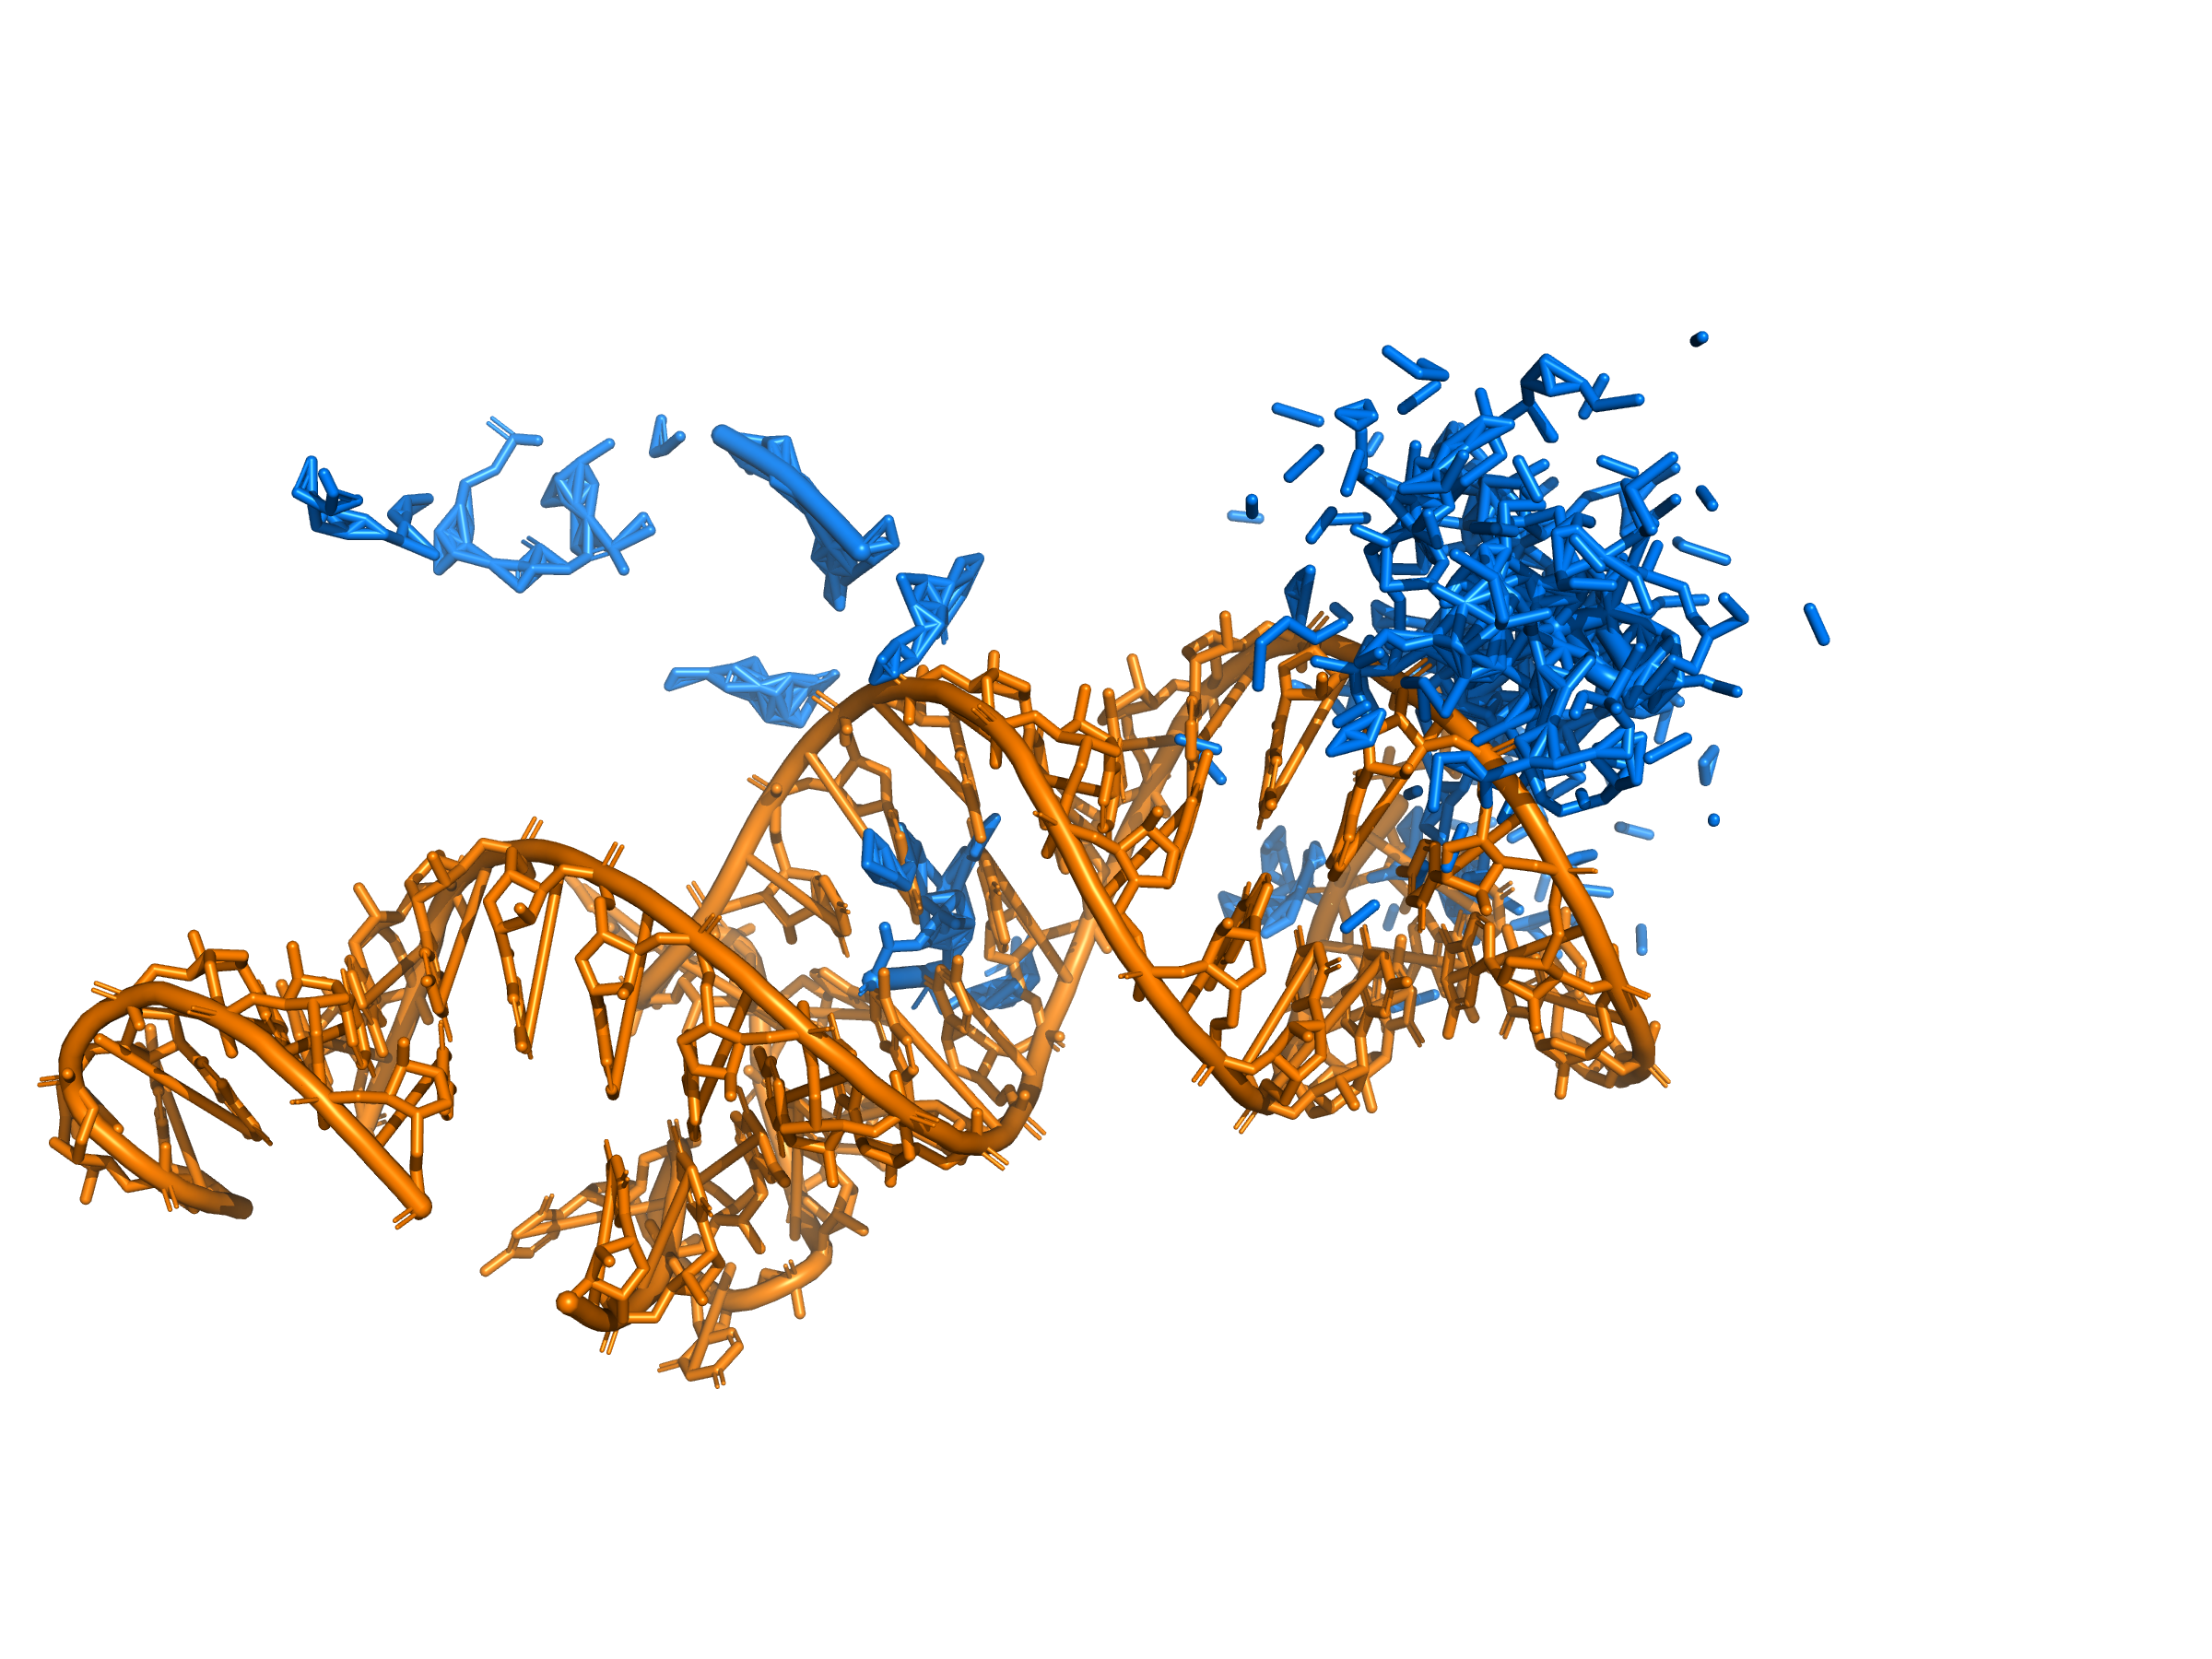
\includegraphics[width=1\linewidth]{img/7w1a_failure.png}
    \caption{Failure case on PDB 7W1A.
Predicted structure (orange) versus native structure (blue) visualized in a non-chain representation due to severe backbone discontinuities in the prediction.}
    \label{fig:placeholder}
\end{figure}